\section{Описание задания и программной реализации}
	\subsection{Краткое описание задания}
		Задание можно разбить на 4 этапа:
		\begin{enumerate}
			\item Generate - генерация графа/портрета по тестовой сетке. По двумерной неструктурированной смешанной сетке, состоящей из треугольников и четырёхугольников генерируется портрет разреженной матрицы смежности графа, дополненный главной диагональю в формате CSR.
			\item Fill - заполнение матрицы и вектора правой части по заданному портрету.
			\item Com - построение схемы обмена данными.
			\item Solve - решение СЛАУ с полученной матрицей. Так как матрица, полученная на предыдущем этапе, симметричная, то используется метод сопряженных градиентов с предобуславливателем Якоби.
			\item Report - проверка корректности и выдача измерений. Проверка, что невязка системы после работы решателя удовлетворяет заданной точности, выдача значения невязки и печать таблицы таймирования всех предыдущих этапов.

		\end{enumerate}

	\subsection{Краткое описание программной реализации}
		Сначала в функции \textit{main} происходит считывание данных командной строки, проверка их корректности и выдача диагностики. Параметры программы: \textit{Nx}, \textit{Ny}, \textit{K1}, \textit{K2}, \textit{Px}, \textit{Py}, их значение хорошо поясняет рисунок \ref{param}, Px и Py - размеры процессорной решётки.
		\begin{figure}[H]
	        \centering
	        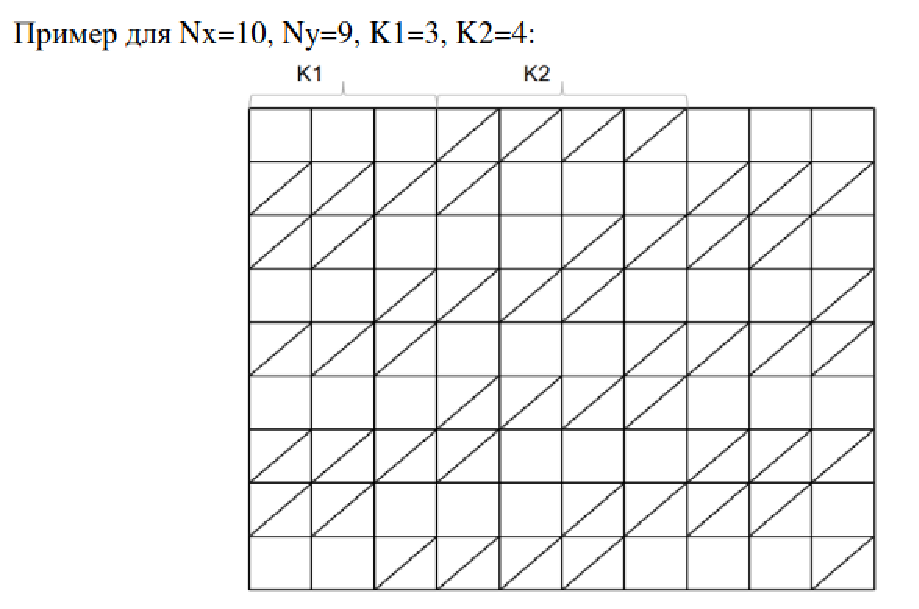
\includegraphics[width=0.5\textwidth]{./images/param}
	        \caption{Параметры командной строки}
	        \label{param}
	    \end{figure}
	    Программа компилировалась mpic++, с флагами -Wall -Wextra -pedantic -std=c++11 -O3 -Wshadow.

	\begin{lstlisting}[numbersep=10pt, language=C++, caption=\textbf{Реализованные функции}]
// Inner product of two vectors vec_1 ans vec_2, N_own - num of own dots
double dotKernel(const int N_own,
                 const std::vector<double>& vec_1,
                 const std::vector<double>& vec_2);

// Linear combination of two vectors x = a * x + b * y
void axpbyKernel(const double a, std::vector<double>& x,
	             const double b, const std::vector<double>& y);

// A function in which the data is treasferred. vec - data vector, com - exchange scheme
void update(std::vector<double>& vec, const Com_struct& com);

// Matrix vector product with sparse matrix. N_own - num of own dots, row_ptr, col_ptr - CSR representation, res = Matrix * vec, com - exchange scheme
void SpMVKernel(const int N_own,
                const std::vector<double>& matrix, const std::vector<int>& row_ptr,
                const std::vector<int>& col_ptr, std::vector<double>& vec,
                const Com_struct& com, std::vector<double>& res);

// Determines whether a cell with the cell_idx index contains oblique line,  K1, K2 - parameters that determine the distribution of oblique lines
bool hasOblique(const int K1, const int K2, const int cell_idx);

// Determines local boundaries, N - side len, p - num of processes, idx - current process index, b, e - begin and end
void get_local_begin_end(const int N, const int p, const int idx, int& b, int& e);

// Function corresponds to the first stage of the task. Nx, Ny, K1, K2, Px, Py- determine the configuration of a two-dimensional grid, rank - rank of the process, size - total processes, N - own + halo, N_own - own, row_ptr, col_ptr - CSR representation, Part - ranks of vertex owners, L2G, G2L - local to global and global to local mapping
void generate(const int Nx, const int Ny,
	          const int K1, const int K2,
	          const int Px, const int Py,
	          const int rank, const int size,
	          int& N, int& N_own, 
	          std::vector<int>& row_ptr,
	          std::vector<int>& col_ptr,
	          std::vector<int>& Part,
	          std::vector<int>& L2G,
	          std::vector<int>& G2L);

// Function corresponds to the second stage of the task. N - own + halo, N_own - own, row_ptr, col_ptr - CSR representation, L2G - local to global mapping, A_arr, b_vec - fillable matrix and vector
void fill(const int N, const int N_own,
          const std::vector<int>& row_ptr,
          const std::vector<int>& col_ptr,
          const std::vector<int>& L2G,
          std::vector<double>& A_arr,
          std::vector<double>& b_vec);

// Building a data exchange scheme. rank - rank of the process, size - total processes, N - own + halo, N_own - own, row_ptr, col_ptr - CSR representation, Part - ranks of vertex owners, L2G, G2L - local to global and global to local mapping, com - exchange scheme
void Com(const int rank, const int size,
         const int N, const int N_own,
         const std::vector<int>& row_ptr,
         const std::vector<int>& col_ptr,
         const std::vector<int>& Part,
         const std::vector<int>& L2G,
         const std::vector<int>& G2L,
         Com_struct& com);

// Function corresponds to the third stage of the task. N - own + halo, N_own - own, A_arr, b_vec - initial data for solving systems of linear equations, row_ptr, col_ptr - CSR representation, x_vec - equations solution, TOL - relative error of the solution
void Solve(const int N, const int N_own, const int rank,
	       const std::vector<double>& A_arr, const std::vector<double>& b_vec,
	       const std::vector<int>& row_ptr, const std::vector<int>& col_ptr,
	       const Com_struct& com, std::vector<double>& x_vec, const double TOL = 1e-7);
\end{lstlisting}

\section{Исследование производительности}
	\subsection{Характеристики вычислительной системы}
	Тестирования программы проводились на вычислительном комплексе \textit{Ломоносов-2}. Ломоносов-2 - массивно-параллельная вычислительная система, состоящая из большого числа вычислительных узлов. Каждый узел оборудован 14 ядерным процессором \textit{Intel Haswell-EP E5-2697v3, 2.6 GHz}, 64 GB оперативной памяти. Узлы связаны сетью Infiniband FDR.
	Некоторые из вычислений выполнены на вычислительном комплексе \textit{IBM Polus}. Polus - параллельная вычислительная система, состоящая из 5 вычислительных узлов. Каждый узел оборудован двумя десятиядерными процессорами \textit{IBM Power 8}, каждое ядро которого имеет 8 потоков, 256 GB оперативной памяти. Производительность кластера (TFlop/s): 55,84 (пиковая), 40,39 (Linpack).
	\subsection{Результаты измерений производительности}
	\subsubsection{Линейный рост времени}
		\begin{table}[H]
			\begin{tabular}{|c||c|c|c|c|c|c|}
				\hline
				\multirow{2}{*}{P} &  \multirow{2}{*}{Generation} & \multirow{2}{*}{Filling} & Dot & Axpby & SpMV          & \multirow{2}{*}{Memory} \\ \cline{4-6}
				                   &                              &                         & \multicolumn{3}{c|}{Solver}  &                         \\ \hline
                \multirow{2}{*}{10000} & \multirow{2}{*}{0.000111} & \multirow{2}{*}{0.000249} & 0.000757 & 0.000098 & 0.000686              & \multirow{2}{*}{} \\ \cline{4-6}
                                       &                     &                    & \multicolumn{3}{c|}{0.001165} &               \\ \hline
                \multirow{2}{*}{100000} &  \multirow{2}{*}{0.001051} & \multirow{2}{*}{0.002475} & 0.004964 & 0.000956 & 0.004021 & \multirow{2}{*}{} \\ \cline{4-6}
                                      &                     &                     & \multicolumn{3}{c|}{0.007286} &  \\ \hline
                \multirow{2}{*}{1000000} &  \multirow{2}{*}{0.010469} & \multirow{2}{*}{0.024775} & 0.044690 & 0.008970 & 0.038380 & \multirow{2}{*}{} \\ \cline{4-6}
                                       &                     &                    & \multicolumn{3}{c|}{0.065353} &  \\ \hline
                \multirow{2}{*}{10000000} &  \multirow{2}{*}{0.107075} & \multirow{2}{*}{0.122159} & 0.106816 & 0.040453 & 0.172713 & \multirow{2}{*}{} \\ \cline{4-6}
                                       &                     &                    & \multicolumn{3}{c|}{0.318858} &  \\ \hline
			\end{tabular}
			\caption{Время (в секундах) работы 3 этапов программы, 3 основных вычислительных ядер для 8 процессов. Polus}
			\label{lineal}
		\end{table}
		По результатам работы можно видеть, что время работы программы растёт линейно. Определить потребляемую память не получилось ни с помощью valgrind, ни по отчёту, выдаваемому планировщиком на Polus, так как он содержит некорректные данные.
		\subsubsection{MPI и OpenMP}
		\begin{table}[H]
			\centering
			\begin{tabular}{|c||c|c|c|c|c|}
				\hline
				\multirow{2}{*}{P / T} &  \multirow{2}{*}{Generation} & \multirow{2}{*}{Filling} & Dot & Axpby & SpMV\\ \cline{4-6}
				                   &                              &                         & \multicolumn{3}{c|}{Solver} \\ \hline
                \multirow{2}{*}{1} & \multirow{2}{*}{|1,00} & \multirow{2}{*}{|1,00} & | 1,00& | 1,00&  | 1,00\\ \cline{4-6}
                                   &                   &                   & \multicolumn{3}{c|}{| 1,00}   \\ \hline
                \multirow{2}{*}{2} & \multirow{2}{*}{|1,00} & \multirow{2}{*}{|0,95} & | 0,95& | 0,50&  | 1,00\\ \cline{4-6}
                                   &                   &                   & \multicolumn{3}{c|}{| 0,9}   \\ \hline
                \multirow{2}{*}{4} & \multirow{2}{*}{|0,97} & \multirow{2}{*}{|0,97} & | 0,95& | 0,45&  | 0,87\\ \cline{4-6}
                                   &                   &                   & \multicolumn{3}{c|}{| 0,80}   \\ \hline
                \multirow{2}{*}{8} & \multirow{2}{*}{|0,93} & \multirow{2}{*}{|0,96} & | 0,92& | 0,37&  | 0,95\\ \cline{4-6}
                                   &                   &                   & \multicolumn{3}{c|}{| 0,75}   \\ \hline
                \multirow{2}{*}{16} & \multirow{2}{*}{|0,62} & \multirow{2}{*}{|0,81} & | 0,52& | 1,9& 0| 0,55\\ \cline{4-6}
                                   &                   &                   & \multicolumn{3}{c|}{| 0,41}   \\ \hline
                \multirow{2}{*}{32} & \multirow{2}{*}{|0,29} & \multirow{2}{*}{|0,58} & | 0,27& | 0,1& 0| 0,26\\ \cline{4-6}
                                   &                   &                   & \multicolumn{3}{c|}{| 0,20}   \\ \hline

			\end{tabular}
			\caption{Эффективность работы 3 этапов программы и 3 основных вычислительных ядер для MPI и OpenMp реализаций, N = 10'000'000, Polus}
			\label{par_1}
		\end{table}
		\subsubsection{Параллельное ускорение}
		\begin{table}[H]
			\centering
			\begin{tabular}{|c||c|c|c|c|c|}
				\hline
				\multirow{2}{*}{P} &  \multirow{2}{*}{Generation | S-up} & \multirow{2}{*}{Filling | S-up} & Dot | S-up & Axpby | S-up & SpMV | S-up \\ \cline{4-6}
				                   &                              &                         & \multicolumn{3}{c|}{Solver | S-up} \\ \hline
                \multirow{2}{*}{1} & \multirow{2}{*}{0,031182 | 1} & \multirow{2}{*}{0,281077 | 1} & 0,029759 | 1 & 0,034563 | 1 & 0,111605 | 1 \\ \cline{4-6}
                                   &                   &                   & \multicolumn{3}{c|}{0,19997 | 1}   \\ \hline
                \multirow{2}{*}{2} & \multirow{2}{*}{0,018937 | 1,65} & \multirow{2}{*}{0,145011 | 1,94} & 0,018165 | 1,64 & 0,015946 | 2,17 & 0,048367 | 2,31\\ \cline{4-6}
                                   &                   &                   & \multicolumn{3}{c|}{0,094317	2,12}   \\ \hline
                \multirow{2}{*}{4} & \multirow{2}{*}{0,010972 | 2,84} & \multirow{2}{*}{0,074735 | 3,76} & 0,010286 | 2,89& 0,008676 | 3,98& 0,030288 | 3,68\\ \cline{4-6}
                                   &                   &                   & \multicolumn{3}{c|}{0,056527 | 3,54}   \\ \hline
                \multirow{2}{*}{8} & \multirow{2}{*}{0,006843 | 4,56} & \multirow{2}{*}{0,037403 | 7,51} & 0,007844 | 3,79& 0,005380 | 6,42& 0,025891 | 4,31\\ \cline{4-6}
                                   &                   &                   & \multicolumn{3}{c|}{0,041447 | 4,82}   \\ \hline
                \multirow{2}{*}{16} & \multirow{2}{*}{0,003879 | 8,04} & \multirow{2}{*}{0,018484 | 15,21} & 0,077089 | 0,39& 0,002268 | 15,24& 0,050457 | 2,21\\ \cline{4-6}
                                   &                   &                   & \multicolumn{3}{c|}{0,091824 | 2,18}   \\ \hline
                \multirow{2}{*}{32} & \multirow{2}{*}{0,002765 | 11,28} & \multirow{2}{*}{0,009300 | 30,22} & 0,126528 | 0,24& 0,001066 | 32,42& 0,062070 | 1,80\\ \cline{4-6}
                                   &                   &                   & \multicolumn{3}{c|}{0,132555 | 1,51}   \\ \hline

			\end{tabular}
			\caption{Время работы и ускорение 3 этапов программы и 3 основных вычислительных ядер, N = 1'000'000, Lom2}
			\label{par_1}
		\end{table}
		\begin{table}[H]
			\begin{tabular}{|c||c|c|c|c|c|}
				\hline
				\multirow{2}{*}{P} &  \multirow{2}{*}{Generation | S-up} & \multirow{2}{*}{Filling | S-up} & Dot | S-up & Axpby | S-up & SpMV | S-up \\ \cline{4-6}
				                   &                              &                         & \multicolumn{3}{c|}{Solver | S-up} \\ \hline
                \multirow{2}{*}{1} & \multirow{2}{*}{0,298306 | 1} & \multirow{2}{*}{2,8935 | 1} & 0,383183 | 1 & 0,374196 | 1 & 0,952436 | 1 \\ \cline{4-6}
                                   &                   &                   & \multicolumn{3}{c|}{1,94348 | 1}   \\ \hline
                \multirow{2}{*}{2} & \multirow{2}{*}{0,164603 | 1,81} & \multirow{2}{*}{1,48933 | 1,94} & 0,197894 | 1,94 & 0,194465 | 1,92& 0,492329 | 1,93 \\ \cline{4-6}
                                   &                   &                   & \multicolumn{3}{c|}{1,00426 | 1,94}   \\ \hline
                \multirow{2}{*}{4} & \multirow{2}{*}{0,0938129 | 3,18} & \multirow{2}{*}{0,747333 | 3,87} & 0,132259 | 2,90& 0,135187 | 2,77& 0,288244 | 3,30 \\ \cline{4-6}
                                   &                   &                   & \multicolumn{3}{c|}{0,603134 | 3,22}   \\ \hline
                \multirow{2}{*}{8} & \multirow{2}{*}{0,0618233 | 4,83} & \multirow{2}{*}{0,373876 | 7,74} & 0,0906956 | 4,22& 0,117391 | 3,19& 0,239105 | 3,98\\ \cline{4-6}
                                   &                   &                   & \multicolumn{3}{c|}{0,484083 | 4,01}   \\ \hline
                \multirow{2}{*}{16} & \multirow{2}{*}{0,0367092 | 8,13} & \multirow{2}{*}{0,18502 | 15,64} & 0,108604 | 3,53& 0,0550623 | 6,80& 0,155744 | 6,12\\ \cline{4-6}
                                   &                   &                   & \multicolumn{3}{c|}{0,303975 | 6,39}   \\ \hline
                \multirow{2}{*}{32} & \multirow{2}{*}{0,0274036 | 10,89} & \multirow{2}{*}{0,093136 | 31,07} & 0,157041 | 2,44& 0,0342204 | 10,93& 0,135025 | 7,05\\ \cline{4-6}
                                   &                   &                   & \multicolumn{3}{c|}{0,275081 | 7,07}   \\ \hline

			\end{tabular}
			\caption{Время работы и ускорение 3 этапов программы и 3 основных вычислительных ядер, N = 10'000'000, Lom2}
			\label{par_2}
		\end{table}
		В таблицах \ref{par_1} и \ref{par_2} представлены время работы параллельной программы на \(1, 2, 4, 8, 16, 32\) процессах, при \(N = 10^6\) и \(N = 10^7\).

		Коммуникации между процессами осуществляются в функциях DOT(allreduce) и SpMV(isend, irecv, wailall), которые испытывают из-за этого проблемы с масштабируемостью. Можно заметить, что производительность начинает падать с 16 процессов и далее, это можно объяснить тем, что для осуществления взаимодействия между процессами появляется необходимость задействовать межузловые связи (на узле максимум 14 процессов), а скорость коммуникаций внутри узла и между узлами отличается примерно на два порядка. Производительность функции DOT начинает уменьшаться с 16 процессов, это происходит из-за того, что в функции производится небольшое количество вычислений, а потом вызывается очень коммуникационно-тяжёлая функция allreduce. Если сравнивать отношения количества вычислений, которые нужно произвести, к количеству данных, которые нужно переслать, для разных размеров задач в функции SpMV, во втором случае оно будет сильно больше, чем в первом, и именно поэтому для большого размера задачи производительность этой функции продолжает расти, несмотря на наличие коммуникаций между узлами. Ещё можно отметить, сверхлинейное ускорение функции AXPBY при \(N = 10^6\), которое происходит из-за небольшого размера производимых вычислений и наличия кэш эффектов.

		\begin{table}[H]
			\begin{tabular}{|c||c|c|c|c|c|c|}
				\hline
				& \multicolumn{6}{|c|}{Nx, Ny, K1, K2} \\ \hline
				   & \multicolumn{3}{c|}{1000, 1000, 10, 5} & \multicolumn{3}{c|}{10000, 1000, 10, 5} \\ \hline
				P  & DOT          & AXPBY        &SpMV  & DOT &AXPBY&SpMV \\ \hline
				1  & 1,94         &2,35          &1,89  & 1,51&2,17 &2,22 \\ \hline
				2  & 3,19         &5,09          &4,37  & 2,92&4,17 &4,29 \\ \hline
				4  & 5,62         &9,36          &6,98  & 4,37&6,00 &7,33 \\ \hline
				8  & \textit{7,38}&15,09         &8,16  & 6,37&6,91 &8,83 \\ \hline
				16 & 0,75         &35,79         &4,19  & 5,32&14,73&13,56 \\ \hline
				32 & 0,46         &\textit{76,15}&3,40  & 3,68&23,70&\textit{15,64} \\ \hline
			\end{tabular}
			\caption{Производительность трёх основных вычислительных ядер, GFlops\\(лучшие результаты выделены курсивом), Lom2}
			\label{real_perf}
		\end{table}
		

\clearpage
%\newpage